\documentclass[conference]{IEEEtran}
%=====PACKAGES=====
\usepackage{amsmath,amssymb}		%To use math symbols
\usepackage{graphicx}				%To include figures
\usepackage[font=footnotesize]{caption}	%To specify the font of captions


%=====SYMBOLS DEFINITIONS=====
\def \R{\mathbb{R}}
\def \X{\boldsymbol{\rm X}}
\def \y{\boldsymbol{\rm y}}
\def \bbeta{\boldsymbol{\beta}}
\def \T{\mathsf{T}}


%=====DOCUMENT=====
\begin{document}
\title{Title of Your Project}
\author{
\IEEEauthorblockN{Team Members' Names}
\IEEEauthorblockA{\sc{CS 4780/6780 Final Project}}
}
\maketitle

%=====ABSTRACT=====
\begin{abstract}
Write abstract here.
\end{abstract}



%=====INTRODUCTION=====
\section{Introduction}
\label{secName}
Here is how you reference Section \ref{secName}. Here is how you cite a paper: \cite{paperName}. Here is how you make a numbered list:
\begin{enumerate}
\item
Here is how you write a scalar: ${\rm x}$.
\item
Here is how you write a vector: $\boldsymbol{\rm x}$.
\item
Here is how you write a matrix: $\boldsymbol{\rm X}$.
\end{enumerate}

Here is how you make a bullet list:
\begin{itemize}
\item
Here is how you write a scalar {\em random} variable: $x$.
\item
Here is how you write a {\em random} vector: $\boldsymbol{x}$.
\item
Here is how you write a {\em random} matrix: $\boldsymbol{A}$.
\end{itemize}

%=====DATA=====
\section{Data}
Here is how you include a Figure:
\begin{figure}[h]
\centering
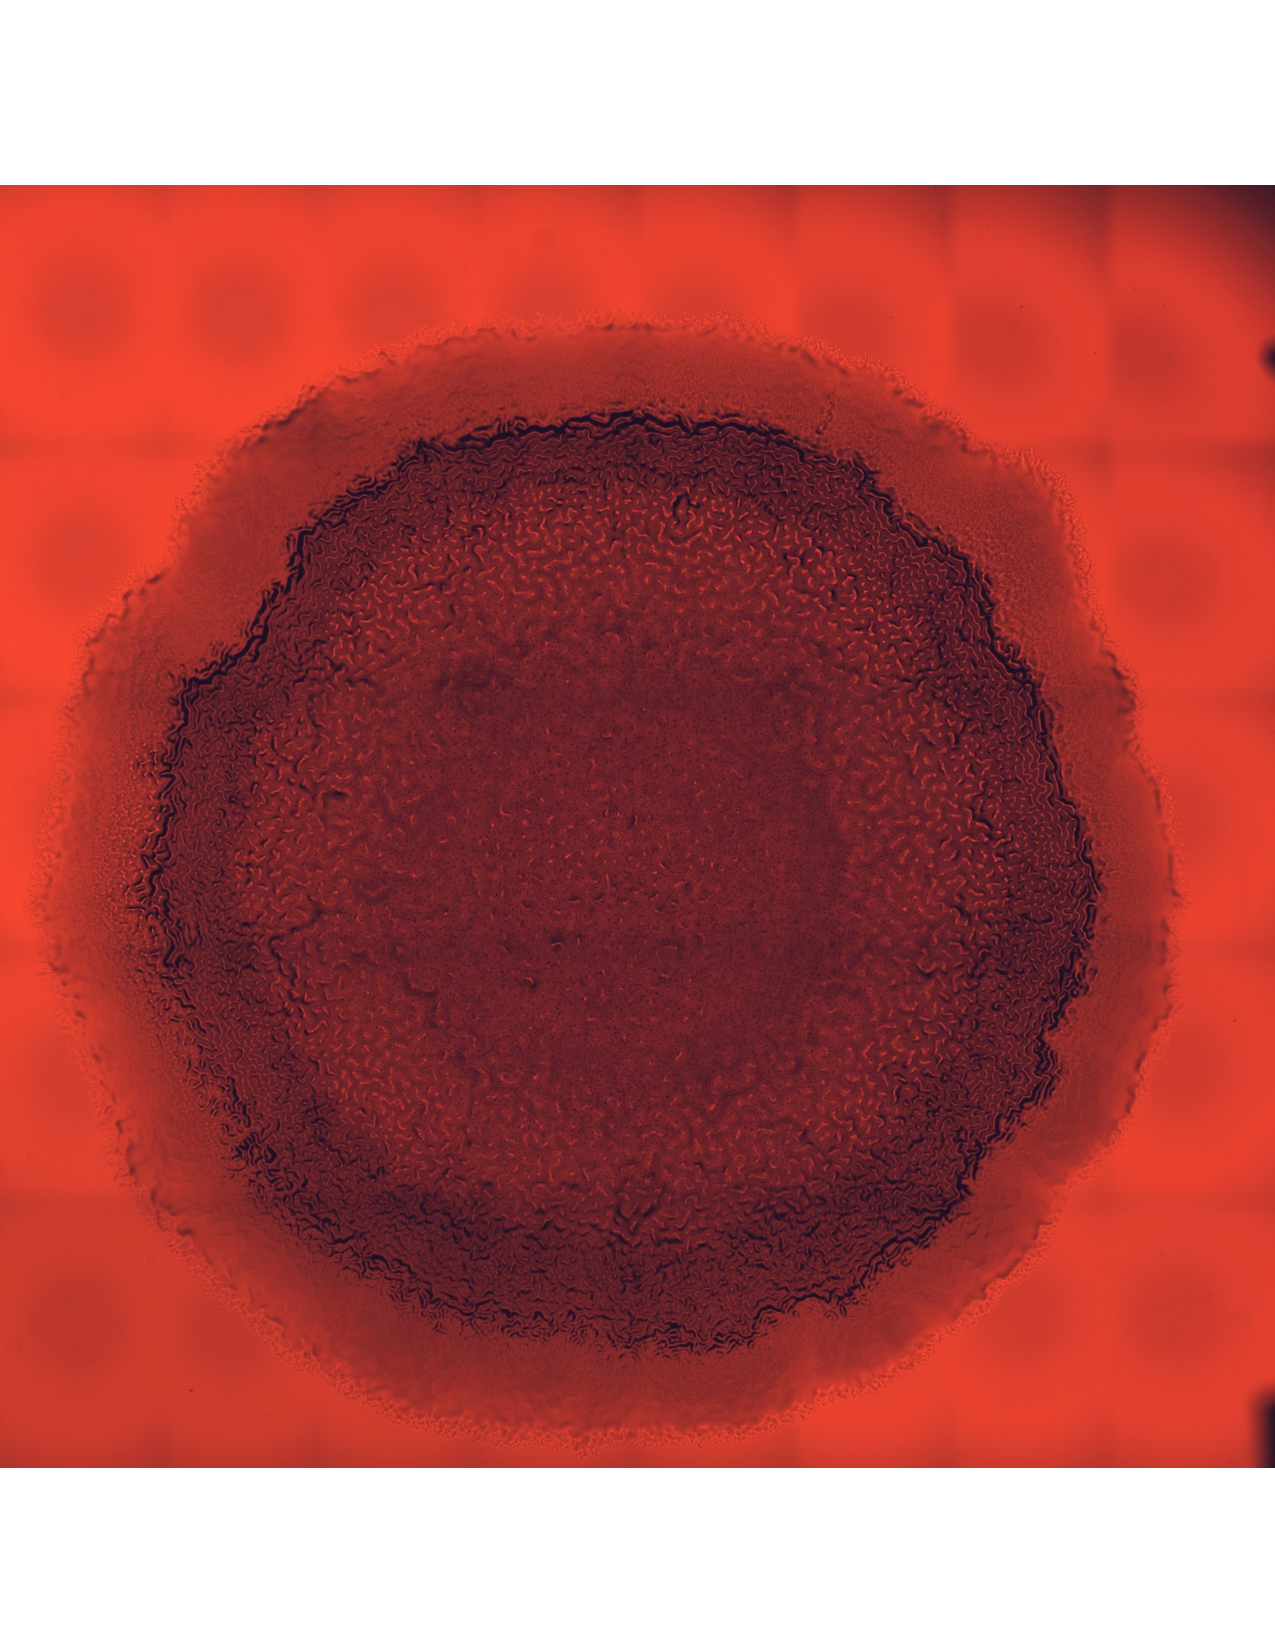
\includegraphics[width=4cm]{Figure_Example.pdf}
\caption{Write Figure's caption here.}
\label{figName}
\end{figure}

Here is how you make a reference to Figure \ref{figName}. Here is how you include a Table:

\begin{table}[h]
\begin{center}
\begin{tabular}{| c || c | c |}
\hline
Image & Antibiotic 1 & Antibiotic 2 \\ \hline \hline
PIL-1\_3dayLBCR-1 & 19 & 4 \\ \hline
PIL-1\_3dayLBCR-2 & 19 & 4 \\ \hline
\vdots & \vdots & \vdots \\ \hline
PIL-373\_3dayLBCR-4 & 24 & 25 \\ \hline
\end{tabular}
\caption{Write Table's caption here.}
\label{tabName}
\end{center}
\end{table}

Here is how you reference Table \ref{tabName}.

%=====METHODS=====
\section{Methods}
Here is how you include an equation:
\begin{align}
\label{eqName}
\bbeta \ = \ (\X^\T\X)^{-1}\X^\T\y.
\end{align}
Here is how you reference equation \eqref{eqName}.



%=====EXPERIMENTS=====
\section{Experiments}
Describe your experiments and present your results.

%=====REFERENCES=====
\begin{thebibliography}{1}

\bibitem{paperName}
D.~Pimentel-Alarc\'on, N.~Boston and R.~Nowak, \emph{Deterministic conditions for subspace identifiability from incomplete sampling}, International Symposium on Information Theory, 2014.

\end{thebibliography}

\end{document}


